\chapter{Apéndice B: Códigos}
\renewcommand{\thepage}{B-\arabic{page}}
\setcounter{page}{1}
    \section{MPPT}
    
        \lstinputlisting[language=C, caption=\texttt{main.c} del MPPT]{main.c}
        \label{Listing B.1}
        
    \section{Etapa de Control}
        \lstinputlisting[language=C, caption=\texttt{main.c} de la Etapa de Control]{maino.c}
        \label{Listing B.2}
        
        \lstinputlisting[language=C, caption=\texttt{gravi.c} de la Etapa de Control]{gravi.c}
        \label{Listing B.3}

        \lstinputlisting[language=C, caption=\texttt{gravi.h} de la Etapa de Control]{gravi.h}
        \label{Listing B.4}

        \lstinputlisting[language=C, caption=\texttt{cap_motor.h} de la Etapa de Control]{cap_motor.h}
        \label{Listing B.5}

        \lstinputlisting[language=C, caption=\texttt{cap_motor.c} de la Etapa de Control]{cap_motor.c}
        \label{Listing B.6}

        \lstinputlisting[language=C, caption=\texttt{cap_sensors.h} de la Etapa de Control]{cap_sensors.h}
        \label{Listing B.7}

        \lstinputlisting[language=C, caption=\texttt{cap_sensors.c} de la Etapa de Control]{cap_sensors.c}
        \label{Listing B.8}

        \lstinputlisting[language=C++, caption=\texttt{main.cpp} de la Etapa de Control]{main.cpp}
        \label{Listing B.9}

        \lstinputlisting[language=Java, caption=\texttt{void loop().java} de la Etapa de Control]{void loop().java}
        \label{Listing B.10}
        
        \begin{figure} [H]
            \centering
            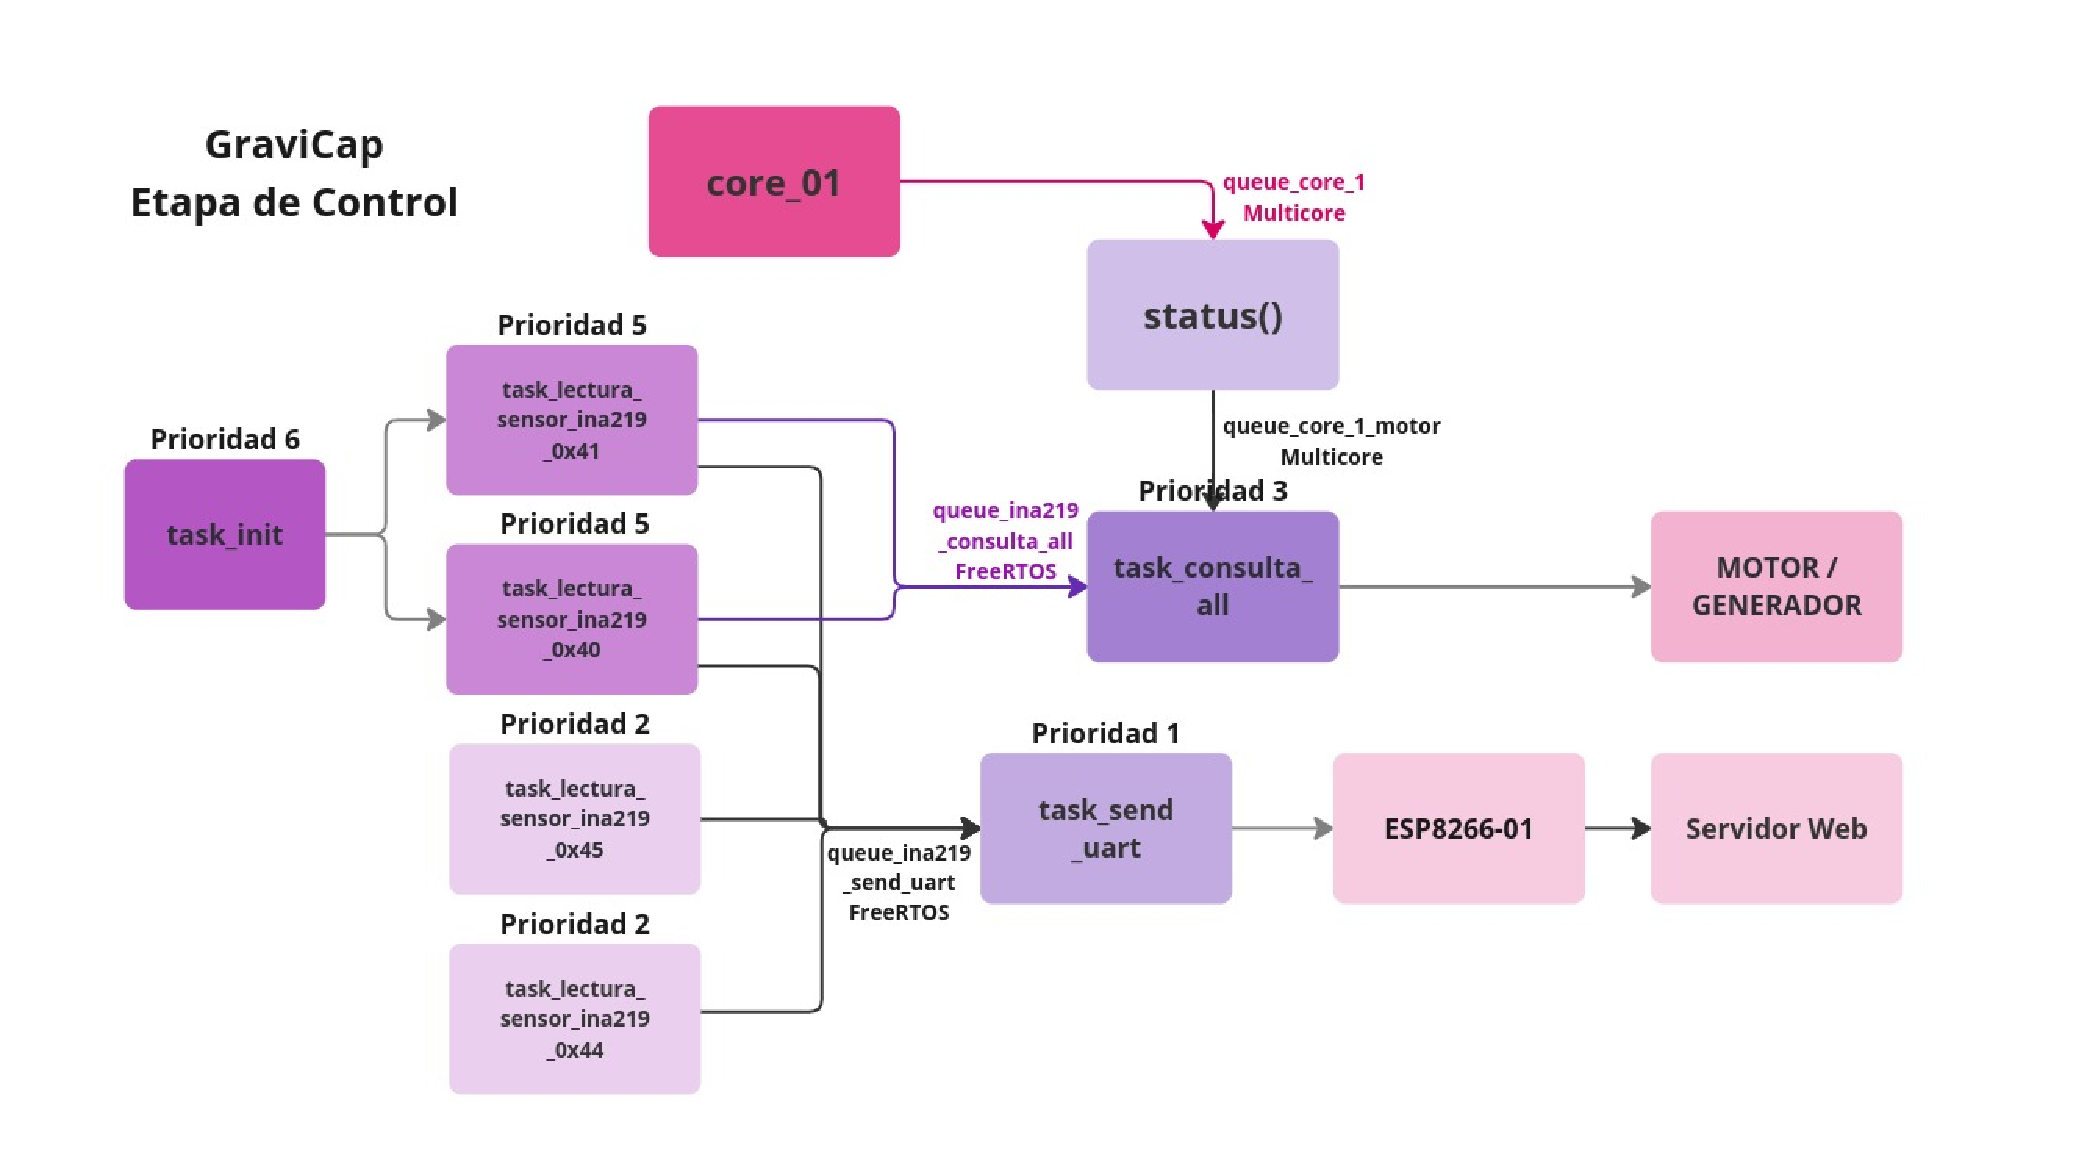
\includegraphics[width=\linewidth]{Imagenes/Anexo_B/Tareas.pdf}
            \caption{Diagrama de Tareas de la Etapa de Control.}
            \label{fig:B1}
        \end{figure}